\documentclass{article}

\usepackage[hidelinks]{hyperref}
\usepackage{enumitem}
\usepackage{listings}
\usepackage{amsfonts}
\usepackage[framemethod = tikz]{mdframed}

\usepackage{geometry}
\geometry{
	a4paper,
	top=3cm,
	bottom=3cm,
	left=2.5cm,
	right=2.5cm,
	heightrounded,
	bindingoffset=0mm
}

\hypersetup{
	colorlinks=false,
	linkcolor=blue,
	filecolor=magenta,
	urlcolor=cyan,
	linktocpage=false
}

\usepackage{titlesec}

\newcommand\chaptername{Section}
\titleformat{\section}[display]{\normalfont\huge\bfseries}{\chaptername\ \thesection}{20pt}{\Huge}
\titlespacing*{\section}{0pt}{50pt}{40pt}
\newcommand\sectionbreak{\clearpage}

\title{ 
	
\includegraphics[width=95mm]{img/PolimiLogo.png} \\
	\bigskip
	Requirements analysis and specification document (RASD)
}

\author{
	Davide Rossetto 894029, Alessandro Tatti 883861
}

\date{
	Delivery date: 2017 May 07\\
	\bigskip v0.6
}

\begin{document}
	
\maketitle
\newpage
\tableofcontents
\newpage
	
	
	\section{Introduction}
	
	
	\subsection{Purpose}
	The Requirements Analysis and Specification Document for the Travlendar+ system management is intended to describe the system itself, its functional and non-functional requirements, its components, its constraints, the relationship with the real world, and users by providing several use cases and scenarios.
	
	A part of the documentation uses Alloy, a language to describe structures and a tool to explore and provide a formal specification of some features of the system.
	
	\bigskip
	This document is predisposed primarily to developers and programmers who must meet the requirements, testers who need to determine if the requirements are met, project managers, who control the development process, and users who validate the goals of the system.
	
	
	\subsection{Scope}
	The product is a digital management system to support the creation of a calendar-based application that automatically computes and accounts for travel time between appointments to make sure that users are not late for appointments and support users in their travels.

	\bigskip
	The system consists of two back -- end server applications:
	\begin{itemize}
		\item An application that handles requests for entering appointments or trips, managing schedules and routes;
		\item An application that communicates with the systems of transportation companies. ***
	\end{itemize}

	\bigskip
	And two front -- end applications:
	\begin{itemize}
		\item The web-based application to provide the end user with a friendly interface to take advantage of services of Travlendar+;
		\item A mobile application that allows the user to easily access the service wherever he needs.***
	\end{itemize}

	\bigskip
	The system is intended for users who must be allowed to register and access the system via username and password, to make the appointment and management process easier and quicker.

	Users can create meetings, and when meetings are created at locations that are unreachable in the allotted time, a warning is created; the application must also take into account possible issues related to the request (e.g. public service strikes on the scheduled day for the meeting). 
	
	\bigskip
	The system should allow users to define various kind of user preferences: user can activate or deactivate each travel means, should be able to provide constraints on different travel means and select combinations of transportation means that minimize carbon footprint. In addition, the user must specify a flexible lunch: the system must handle this, allowing the user to have half an hour to have lunch within the set time interval.
	
	
	\subsection{Goal}
	The goals of Travlendar+ are the followings:

	\begin{enumerate}
		\item Let the user register to the service and login via provided credentials;
		\item Let the user manage his/her own profile;
		\item Let the user insert his/her meeting in the schedule application;
		\item Let the system work efficiently by generating an alarm when a meeting is not possible within the specified time range;
		\item Let the system indicate which best travel means is to be used for a given meeting;
		\item Let the user indicate his/her preferences on the travel means;
		\item Automatically the system searches for the shortest path to reach the meeting site;
		\item Automatically the system searches the cheapest means of transport to reach the meeting site;
		\item Let the user specify a flexible lunch, i.e. a period of time to eat;
		\item Let the user specify its intent to minimize his carbon footprint;
		\item Automatically the system must find at least half an hour to have lunch (within the "flexible lunch" time).
	\end{enumerate}

	
	\subsection{Definitions, Acronyms, Abbreviations}
	\begin{description}
		\item[Actor:] Specifies a role played by a user or any other system that interacts with the system;
		\item[API: ]Application Programming Interfaces.
		\item[Back -- end application:] Computer program that remains in the background, or resides on a server located in a back room. A user, generally, interfaces only with a front -- end application.
		\item[Front -- end application:] Any application the users interact with directly. It provides the so called presentation layer.
		\item[GPS:] Global Positioning System
		\item[Guest:] Any person who is not registered or logged in to the Travlendar+ service.
		\item[JEE:] Java Enterprise Edition
		\item[Mobile application:] Computer program designed to run on a mobile device such as smartphone or tablet.
		\item[OS:] Operative system.
		\item[RASD:] Requirements Analysis and Specification Document.
		\item[System:]
		\item[User:] Any person subscribed and logged in to the service who hence can insert a meeting using Travlendar+.
		\item[User Interface:] It is the way through which a user interacts with an application or a website.
		\item[Web application:] Client -- server application accessible by an user through a browser.
	\end{description}
	
	
	\subsection{Revision history}
	\begin{description}
		\item[v0.1] Construct basic document's structure.
		\item[v0.2] Add \textit{Purpose}, \textit{Scope}, \textit{Goal}, \textit{Definitions, Acronyms, Abbreviations}, \textit{Reference documents}, \textit{Document structure}.
		\item[v0.3] Add \textit{Product Perspective}, \textit{Product Functions}, \textit{User Characteristics}, \textit{Assumptions and Dependencies}, \textit{Constraints}, \textit{World and Machine model interpretation}. Modify \textit{Definition, Acronyms, Abbreviations} and document structure. Create a simple Appendix, that will be completed at the end.
		\item[v0.4] Add \textit{External Interface Requirements}. Modify \textit{Goal}, \textit{Definitions, Acronyms, Abbreviations}, \textit{Product Functions}, \textit{Use Case Model}, \textit{Assumption and Dependences}, \textit{World and Machine model}.
		\item[v0.5] Add \textit{Functional Requirements}.
		\item[v0.6] Add \textit{Performance Requirements} and \textit{Software System Attributes}.
	\end{description}
	
	
	\subsection{Reference documents}
	This document is based on the specifications concerning the RASD assignment for the Software Engineering II project, part of the course held by professors Elisabetta Di Nitto and Matteo Giovanni Mottola at the Politecnico di Milano, A.Y. 2017/2018.
	
	
	\subsection{Document structure}
	This document consists of three sections:

	\begin{description}
		\item[Section 1: Introduction] A general introduction and overview of the system-to-be purpose, scope and goals, along with some important information about this document.
		\item[Section 2: Overall description] It describes the general factors that affects the product and its requirements. The section provides a background for those requirements which are defined in detail in Section 3 and makes them easier to figure out.
		\item[Section 3: Specific Requirements] All the software requirements are specified to a level of detail which is sufficient to let the designers satisfy them. Both functional and non-functional requirements are mentioned.
	\end{description}
	
	\bigskip
	There are two additional parts, Appendix and Bibliography that provide another information about the sections of this document.
	
	\section{Overall Description}	
	
	
	\subsection{Product Perspective}
	
	
	\subsubsection{User interfaces}
	The user have two main ways to access the system:
	\begin{itemize}
		\item through a web application accessible from any modern browser
		\item through a mobile application that can run on any modern smartphone
	\end{itemize}
	Although they are two different platforms, the user interface must be unified and intuitive, allowing anyone to use it without any training needed.


	\subsubsection{Hardware interfaces}
	The web application can be executed on any modern computer that meets the minimum system requirements (link al paragrafo).
	
	\bigskip
	The mobile application can run on any modern mobile device (i.e. smartphone, tablet) with mobile data connectivity,  GPS and meets the minimum system requirements (link al paragrafo).


	\subsubsection{Software interfaces}
	The web application must support most of the modern browsers e.g., IE, Firefox, Chrome, Safari.
	
	\bigskip
	The mobile application must be supported by the most widespread mobile OSs such as iOS and Android that meets the minimum system requirements (link al paragrafo).

	\bigskip
	The backend application must rely on a commercial DBMS to store data and must be implemented in Java.
	The backend also have to interface with the APIs of a public transportation and  traffic informations provider.***
	
	
	\subsection{Product Functions}
	The system allows the users to create meetings, helps them to reach the location.
	
	The users can:
	\begin{itemize}
		\item register to the service;
		\item login in to the service;
		\item manage personal information and delete their accounts;
		\item create meetings;
		\item manage their preferences, such as activate/deactivate travel mean, provide constraints on travel mean, specify their intent to minimize his carbon footprint;
		\item specify lunch time.
	\end{itemize}
	
	\bigskip
	\bigskip
	\begin{figure}[htbp]
		\begin{center}
		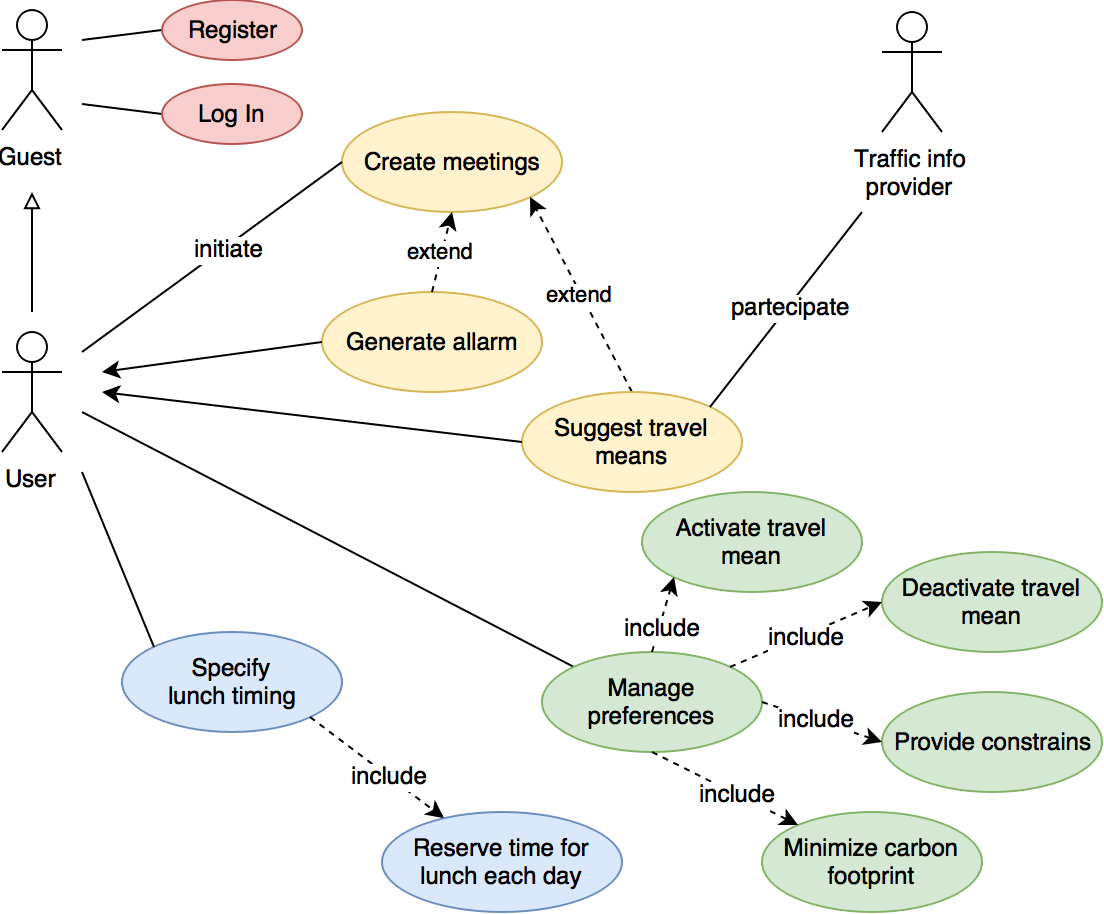
\includegraphics[width=0.75\textwidth]{img/UseCaseModel.png}
		\caption{Use Case Model. Explains actors and functionalities offered by the system.}
		\label{default}
		\end{center}
	\end{figure}
	
	
	\subsection{User Characteristics}
	The target user is someone who needs an automated system to manage appointments that also handle the scheduling of travels.
	
	The meeting should not overlap with any pre-existing one and should allow the user to move from his/her current position to the meeting position, according with preferred travel means and traffic conditions.
	
	
	\subsection{Assumptions and Dependences}
	The following assumptions are given for granted:
	\begin{itemize}
		\item  Transport means are complied with the user's request.
		\item  Device is always connect to the server.
		\item  All users provided correct and valid data at time the registration.
		\item  GPS shows the actual position of the owner.
		\item  Provider Information shows correct and update data.
		\item  The event, when it's inserted, must not be in the past.
	\end{itemize}
	
	
	\subsection{Constraints}
	
	
	\subsubsection{Regulatory policies}
	The application must be allowed by the user to collect his/her position, through GPS.
	
	
	\subsubsection{Hardware limitations}
	\begin{itemize}
		\item Web application:
			\begin{itemize}
				\item Internet connection;
				\item 800x600 screen resolution;
				\item JavaScript enabled.
			\end{itemize}
		\item Mobile application:
			\begin{itemize}
				\item Internet connection;
				\item 50 MB of available storage space;
				\item 1GB of RAM;
				\item GPS module.
			\end{itemize}
	\end{itemize}
	
	
	\subsubsection{Reliability requirements}
	The system reliability, that is the probability to operate without a failure for a specific period of time, must be at least 99\%.
	
	
	\subsection{World and Machine model interpretation}
	In this part of RASD, a description of the system-to-be is provided following the World and Machine model introduced by Jackson and Zave.
	
	\bigskip
	They indicate as the Machine the portion of the system to be developed, typically software-to-be plus hardware. The Machine domain is the set of phenomena located entirely in the machine and that the machine control (e.g., machine algorithms, controlled device, ...)
	
	\bigskip
	Opposite, the World domain is a set of phenomena that the machine cannot observe.

	\bigskip
	The World is connected with the Machine through Shared Phenomena--part can be observable both by the Machine and by the World. The Shared Phenomena can be controlled by the world and observed by the Machine or controller by the machine and observe by the world.
	
	\bigskip
	\bigskip
	\begin{figure}[htbp]
		\begin{center}
		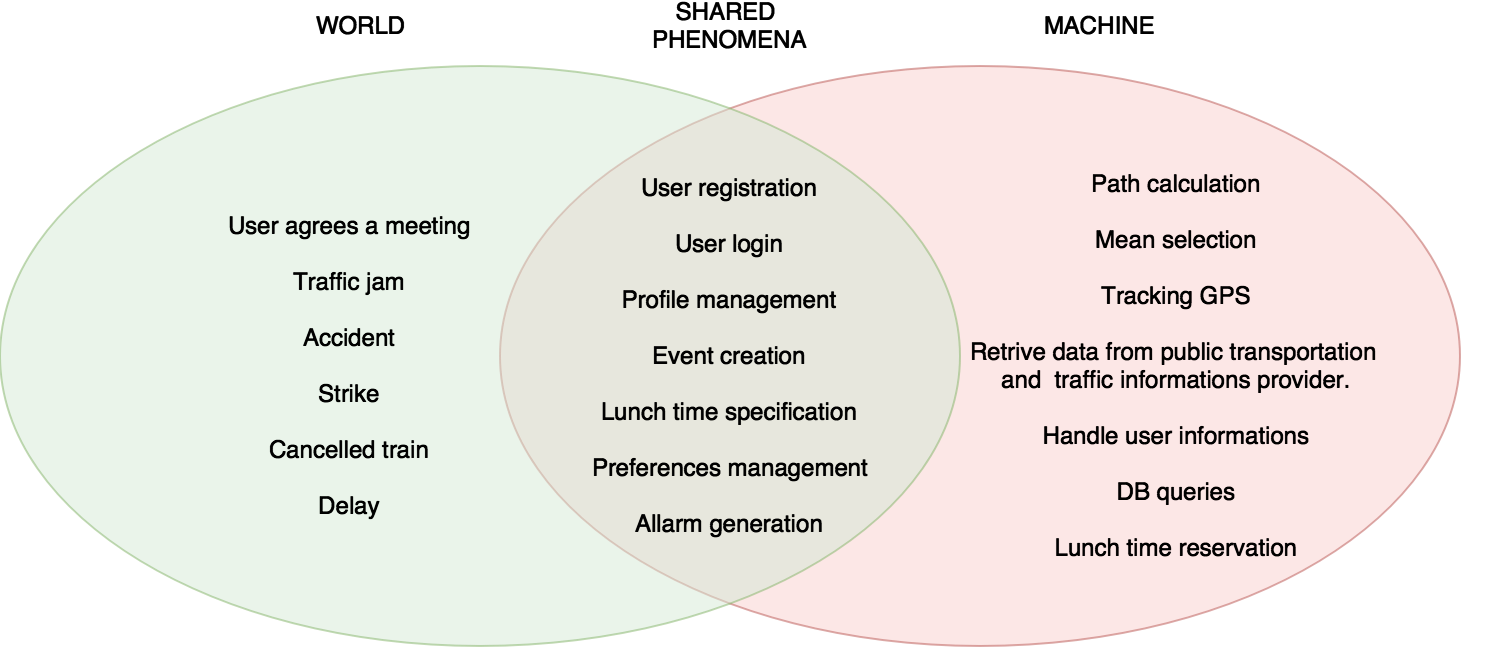
\includegraphics[width=\textwidth]{img/WorldAndMachineModel.png}
		\caption{World and Machine model for the main functionalities offered by the system.}
		\label{default}
		\end{center}
	\end{figure}

	
	\section{Specific Requirements}
	
	
	\subsection{External Interface Reqirements}
	
	
	\subsubsection{User Interfaces}
	The user interface must be intuitive and unified, granting to the user a pleasant experience. In order to make it possible both web and mobile application must satisfy the following requirements:
	\begin{itemize}
		\item If the session is not already active the user must be redirected to a Login page. If he/she is not already registered he/she can create a new account within the same page. Moreover, the user must be able to Sign In/Sign Up not only with username and password but also with his/her social accounts (e.g. Google, Facebook, Twitter);
		\item Once logged, the user must be redirected to his/her personal page;
		\item A toolbar must allow the user to navigate through the pages described below;
		\item The user's personal page must display an overview of user's future events (display them in a list or in a calendar view) and must also offer the possibility to insert new ones;
		\item Clicking on an event the user must be redirected to the event's detail page;
		\item The event's detail page must display detailed information such as location of the event, time and suggested mean (including the path)  needed to reach it;
		\item The event's detail page must allow the user to modify or delete the event;
		\item If an user tries to inserted or modified an event which location is unreachable in the remaining time an alert should be displayed;
		\item The Account settings page must allow the user to modify its/her personal informations or delete the account;
		\item The user must be allowed to select between different languages (en, it, de, fr, es, ru, zh, ja, ar);
		\item The UI must comply the Flat Design principles;
		\item Both web and mobile applications must use the same graphic objects for the same interface elements.
	\end{itemize}
	
	\bigskip
	\bigskip
	Specific constraints must be satisfied by specific application:
	\begin{itemize}
		\item Web application:
			\begin{itemize}
				\item The user interface must be responsive i.e. adapt to screen size;
				\item All pages must comply W3C standards.
			\end{itemize}
		\item Mobile application:
			\begin{itemize}
				\item Must run on iOS 9.3 or greater and Android 5.0 or greater.
			\end{itemize}
	\end{itemize}

	
	
	\subsubsection{Hardware Interfaces}
	As already mentioned in section 2.1.2, the web application can be executed on any computer that meets the basic requirements described in the "Hardware Limitation" section.
	
	\bigskip
	The mobile application must exchange data with the GPS module located on any type of smartphone or tablet. You must also have an internet connection to communicate with the main system server.

	
	\subsubsection{Software Interfaces}
	The backend application requires the following software products:
	\begin{itemize}
		\item Java EE 7 - http://www.oracle.com/technetwork/java/javaee/overview/index.html
		\item MySQL 5.7 - http://dev.mysql.com/
	\end{itemize}
	
	\bigskip
	As mentioned in Section 2.1.3, the backend must interfaced with the APIs of a public transportation and  traffic informations provider, to have the information useful to plan the path.
	
	\bigskip
	The mobile applications requires the following software products:
	\begin{itemize}
		\item (iOS) Swift 4 - https://developer.apple.com/swift/
		\item (Android) Java SE 7 - http://www.oracle.com/technetwork/java/javase/overview/index.html
	\end{itemize}

	
	\subsubsection{Communications Interfaces}
	Every communication between application server and client must comply the HTTPS protocol.
	
	\bigskip
	If the back-end application and the DBMS runs on different servers the communication between them must be SSL/TLS encrypted.
	
	
	\subsection{Functional requirements}
	
	
	\subsubsection{Register}
	
	\bigskip
	\noindent
	\textbf{Purpose} \\
	Anyone who want to subscribe to Travlendar + can make the registration process through the mobile app or the web site.
First, the guest must complete the registration form with personal data (i.e., first name, last name, birthdate, sex, mail, password) and accept privacy terms and conditions.

	Once the guest submits the information, the system checks and sends a confirmation email. If the operation is successful, the guest becomes a user and may start using the application.
	
	\bigskip
	\noindent
	\textbf{Scenario 1} \\
	Allyson wants to register at Travlendar + using the web page. She opens the main home page of research mean and type "travlendar +". When you reach Travlendar's home page, click on SignUp and the registration form appears. It inserts all your data, such as first name, last name, birthdate, sex, email and password, and accepts the terms and conditions of privacy. When you finish this step, click the Submit button, and after a few seconds you will receive a confirmation email of your registration.

	\bigskip
	\noindent
	\textbf{Scenario 2} \\
	Benjamin has just moved to London and, at the suggestion of his friend Carl, decides to sign up for Travlendar + to better manage new meetings. Download the app on your mobile phone and open it. The home page appears and he clicks on SignUp. The registration form appears where he inserts all personal information and clicks "Submit" button to submit it. Just click the button will display a message informing him that his password has already been used.
	
	\bigskip
	\noindent
	\textbf{Use cases} \\

	\begin{table}[htp]
	\caption{Register use case.}
		\begin{center}
    			\begin{tabular}{p{0.3\textwidth}|p{0.6\textwidth}}
   			 	\hline
    				Actor & Guest \\ \hline
    				Goal & Goal 1 \\ \hline
    				Input Condition & The person wants to subscribe to the service \\ \hline
    				Event flow & 
				\begin{enumerate}
  					\item The guest opens the home page or mobile application of "Travlendar +"  and clicks the "SignUp" button;
  					\item The registration form appears and the guest completes the mandatory fields;
  					\item The guest allows the personal data processing to be marked on the corresponding box;
  					\item The guest clicks the "Submit" button;
  					\item The system saves the information in the database and sends a guest confirmation email to the guest, who becomes a user of the service.
 				 \end{enumerate} \\ \hline
    				Output Condition & The system informs the user of the registration successfully. \\ \hline
    				Exception & The system can report some exceptions when an invalid or already used mail address is used. Another exception can be reported if the license number is non-existent or if the terms and conditions of use are not accepted. \\ \hline
    			\end{tabular}
		\end{center}
	\end{table}
	
	
	\bigskip
	\noindent
	\textbf{Activity diagram} \\
	
	
	\bigskip
	\noindent
	\textbf{Functional requirements} \\
	
	\begin{itemize}
		\item The system must not accept a mail already used for the registration process;
		\item The system requires the following mandatory personal information:
			\begin{itemize}
				\item First Name
				\item Last Name
				\item Sex
				\item Date of birth
				\item Address
				\item E-mail address
				\item Password
				\item Driving license number (optional)
			\end{itemize}
		\item If the terms and conditions of use and privacy are not accepted, the system must not complete the registration process;
		\item The system sends a recording confirmation mail correctly, when the guest clicks the "Submit" button;
		\item The guest can leave the registration process at any time.
	\end{itemize}

	\subsubsection{Login}
	
	\bigskip
	\noindent
	\textbf{Purpose} \\
	The purpose of the Login phase is to guarantee access to authorized users. Access can be made by inserting mail and password, or through a social network account (i.e., Facebook, Instagram, Linkedin).

	It is also possible to retrieve password if it has been forgotten by clicking the "Forgot Password?" button. Once the button is clicked, a mail with credentials is sent.

	\bigskip
	\noindent
	\textbf{Scenario 1} \\
	Catherine wants to enter a new meeting in her calendar. Catherine accesses the "Travlendar +" home page with her laptop. Enter personal mail and password (used to sign up). Then you click on "Login" and, since everything is correct, you get access as an authorized user.
	
	\bigskip
	\noindent
	\textbf{Scenario 2} \\
	Dominique wants to insert his dental visit on next Tuesday. Opens the app on your mobile phone and places credentials. Now there is a problem, you do not remember the password used to authenticate yourself. Then, Dominique click on the "Forgot Password?" button. The system forwards the new password to its email address to be used to authenticate itself.
	
	\bigskip
	\noindent
	\textbf{Use cases} \\
	
	\begin{table}[htp]
	\caption{Purpose use case.}
		\begin{center}
    			\begin{tabular}{p{0.3\textwidth}|p{0.6\textwidth}}
   			 	\hline
    				Actor & User \\ \hline
    				Goal & Goal 1 \\ \hline
    				Input Condition & An  user already registered, wants to login. \\ \hline
    				Event flow & 
				\begin{enumerate}
  					\item The user opens the home page or mobile application and the system shows the login page;
  					\item The user inserts his / her mail address and password;
  					\item The user clicks the "Login" button.
 				 \end{enumerate} \\ \hline
    				Output Condition & The system connects the user to his / her personal page. \\ \hline
    				Exception &The exception that may arise is the inputting of an insertion mail or an incorrect password. The system sends the user an error message asking you to verify the address and re-enter the password. \\ \hline
    			\end{tabular}
		\end{center}
	\end{table}
	
	\bigskip
	\noindent
	\textbf{Activity diagram} \\
	
	
	\bigskip
	\noindent
	\textbf{Functional requirements} \\
	\begin{itemize}
		\item The user must be already registered with the system for successful login;
		\item You must have correct mail and password available to successfully login;
		\item The user-entered password must match a specific mail address;
		\item Bad credentials must not allow the user authentication;
		\item The system must send a new password to the specified mail attachment (if this is valid), if the user clicks the "Forgot Password?" button;
		\item After requesting a new password, the system must allow the user to authenticate only with new credentials.
	\end{itemize}

	\subsubsection{Create meetings}
	
	\bigskip
	\noindent
	\textbf{Purpose} \\
	The purpose is to allow the authorized user to create a new meeting on the calendar by entering the meeting name, date, time, place, and also specifying how to reach the site. The task of the system is to check this information and, if incorrect, alert the user to modify them.
	
	\bigskip
	\noindent
	\textbf{Scenario 1} \\
	Emma has to enter a driving lesson for tomorrow. Then she logs in her "Travlendar +" personal page as authorized user and press the "+ New" button to create the appointment. Then the system open a form where she must enter the name of the event, date, time, place and mode to reach it. Once completed, you press the "Save" button. The system verifies the correctness of the information and creates the event on the calendar.
	
	\bigskip
	\noindent
	\textbf{Scenario 2} \\
	Franklin just took an appointment from the hairdresser in half an hour. She then decided to create an appointment on her mobile app "Travelendar +". Log in with your smartphone and press the "+ New" button. A form appears to be completed with the event, date, time, place and mode to reach it. Franklin wants to use a bike sharing service. Once the form is completed, submit it. The system checks the information and issues an error message because the site can not be reached in half an hour by bike.
	
	\bigskip
	\noindent
	\textbf{Use cases} \\
	
	\begin{table}[htp]
	\caption{Create meetings use case.}
		\begin{center}
    			\begin{tabular}{p{0.3\textwidth}|p{0.6\textwidth}}
   			 	\hline
    				Actor & User \\ \hline
    				Goal & Goal 4 \\ \hline
    				Input Condition & An user wants to create a new meeting on his/her calendar.\\ \hline
    				Event flow & 
				\begin{enumerate}
  					\item The user must login by entering his/her mail and password;
  					\item The user clicks the "+ New" button to create a new meeting;
  					\item The system shows the form to be filled;
  					\item The user compiles the form and clicks the "Save" button;
  					\item The system checks the information and saves it in the database; in the case of incorrect information, the user alerts you with an error message.
 				 \end{enumerate} \\ \hline
    				Output Condition & The system creates a new meeting on the user's calendar in the home page. \\ \hline
    				Exception & The exception that may emerge is that the mean to reach the site is not valid (e.g., if you have to drive a motorway, you cannot use the bicycle), or your downtime is less than the time you need. Another exception is raised if the meeting creation date is later than the date of the meeting. \\ \hline
    			\end{tabular}
		\end{center}
	\end{table}
	
	\bigskip
	\noindent
	\textbf{Activity diagram} \\
	
	
	\bigskip
	\noindent
	\textbf{Functional requirements} \\
	\begin{itemize}
		\item The user must log in successfully;
		\item The user must insert the following information in the form:
			\begin{itemize}
				\item Meeting name
				\item Meeting data
				\item Meeting Time
				\item Place
				\item People
				\item Transport modes
			\end{itemize}
		\item The system must verify that the meeting data is later than the creation date;
		\item The system must check that the way to reach is compatible with the path;
		\item The system must verify that the time available is sufficient to reach the appointment site;
		\item After verification of the correctness of the information, the system must create the meeting on the personal calendar;
		\item The system must send an error message in case of inappropriate data or mean.
	\end{itemize}

	\subsubsection{Modify meetings}
	
	\bigskip
	\noindent
	\textbf{Purpose} \\
	The purpose of this part is to allow the user, after saving an meeting on the calendar, to be able to modify some information (such as date, time, number of people, place, means of transport). The system must verify the compatibility of the modification.
	
	\bigskip
	\noindent
	\textbf{Scenario 1} \\
	Gordon was just called by the school secretary and was advised that he had a lesson in IIIA class at 10 a.m. instead of at 9 a.m. on Thursday. Enter the personal page of "Travlendar +" and select the appointment. Press the "Modify" button next to the selected event. The system shows the form already completed and Gordon changes the time. Press the "Save" button. The system checks the information and updates the appointment successfully.
	
	\bigskip
	\noindent
	\textbf{Scenario 2} \\
	Helen has to hold a conference in Paris. Now she is at Milan Malpensa Airport and she has just been notified that the plane has 120 minutes late. He decides to change the meeting to control if she can reach the conference place in time. Enter your personal page through the mobile application. Helen selects the meeting and press the "Modify" button. Then, she change the times in the form and press "Save". The system verifies the information and sends an error message because by changing the time the plane will fail to reach Paris in time for the conference.
	
	\bigskip
	\noindent
	\textbf{Use cases} \\
	
	\begin{table}[htp]
	\caption{Modify meetings use case.}
		\begin{center}
    			\begin{tabular}{p{0.3\textwidth}|p{0.6\textwidth}}
   			 	\hline
    				Actor & User \\ \hline
    				Goal &  Goal 5 \\ \hline
    				Input Condition & The user wants to modify a meeting on his/her calendar. \\ \hline
    				Event flow & 
				\begin{enumerate}
  					\item The user must login by entering your mail and password;
  					\item The user selects the meeting he/she wants to modify with one click;
  					\item The system shows a dialog box with "Modify" and "Delete" buttons;
  					\item The user presses the "Modify" button;
  					\item The system shows the form with the meeting information;
  					\item The user modifies the form and press the "Save" button;
  					\item The system verifies the information and saves it in the database; in the case of incorrect information, the system alerts the user with an error message.
 				 \end{enumerate} \\ \hline
    				Output Condition & The system modify a meeting on the calendar on the user's home. \\ \hline
    				Exception & The exceptions that can be raised are the same as those for creating the event. The exception that may be raised is that the way to reach the site is not valid (for example, if you have to drive a motorway, you can not use the bicycle), or your downtime is less than the time you need. Another exception is raised if the meeting change date is later than the date of the meeting. \\ \hline
    			\end{tabular}
		\end{center}
	\end{table}
	
	\bigskip
	\noindent
	\textbf{Activity diagram} \\
	
	
	\bigskip
	\noindent
	\textbf{Functional requirements} \\
	\begin{itemize}
		\item The user must log in successfully;
		\item The user must have already created an event;
		\item The user must change one or more of the following information in the form:
			\begin{itemize}
				\item Event name
				\item Event date
				\item Event Time
				\item Place
				\item People
				\item Transport modes
			\end{itemize}
		\item The system must verify that the date of the event is after the creation date;
		\item The system must check that the way to reach is compatible with the path;
		\item The system must verify that the time range is sufficient to reach the appointment place;
		\item Once the information is verified, the system has to change the appointment on the personal calendar;
		\item The system must send an error message in case of inappropriate date or time.
	\end{itemize}


	\subsubsection{Delete meetings}
	
	\bigskip
	\noindent
	\textbf{Purpose} \\
	The purpose of this part is to allow the user, after creating or modifying an meeting on the calendar, to be able to delete it.
	
	\bigskip
	\noindent
	\textbf{Scenario 1} \\
	Igor is a computer science student. On Monday and Tuesday he attends the course of Database 2. The professor has just written an e-mail, signaling that next Monday there will be no lesson. Igor opens the "Travlendar +" application on his smartphone and he logs in. He selects the "DB2 lesson" meeting and clicks the "Delete" button. The system asks whether he is sure to cancel the meeting. Igor confirms. The system processes the information and updates the database.
	
	\bigskip
	\noindent
	\textbf{Use cases} \\
	
	\begin{table}[htp]
	\caption{Delete meetings use case.}
		\begin{center}
    			\begin{tabular}{p{0.3\textwidth}|p{0.6\textwidth}}
   			 	\hline
    				Actor & User \\ \hline
    				Goal & Goal 6 \\ \hline
    				Input Condition & The user wants to delete a meeting on his/her calendar. \\ \hline
    				Event flow & 
				\begin{enumerate}
  					\item The must login by entering your mail and password;
  					\item The user selects the meeting he/she wants to select with one click;
  					\item The system shows a dialog box with two "Modify" and "Delete" buttons;
  					\item The user clicks the "Delete" button;
  					\item The system prompts the user if he/she is sure he/she want to delete the meeting with a dialog box;
  					\item The user presses the "Yes" button;
  					\item The system processes the information, updates the database, and deletes the event from the calendar.
 				 \end{enumerate} \\ \hline
    				Output Condition & The system deletes a meeting on the user's home calendar. \\ \hline
    				Exception & The delete fails and the user is notified. \\ \hline
    			\end{tabular}
		\end{center}
	\end{table}
	
	\bigskip
	\noindent
	\textbf{Activity diagram} \\
	
	
	\bigskip
	\noindent
	\textbf{Functional requirements} \\
	\begin{itemize}
		\item The user must log in successfully;
		\item The user must have already created a meeting;
		\item The user must select the meeting he/she wants to delete;
		\item The system must ask the user whether or not he/she want to delete the meeting;
		\item The system must update the DB and delete the meeting from the calendar.
	\end{itemize}


	\subsubsection{Manage profile informations}
	
	\bigskip
	\noindent
	\textbf{Purpose} \\
	Both web and mobile applications must allow the user to view and update some personal informations coherently with the provided constraints.
	
	\bigskip
	\noindent
	\textbf{Scenario 1} \\
	Karlie, due to a problem with her e-mail services provider, wants to change her e-mail address. Karlie opens a browser window, reaches the Travelendar+ homepage and logs in. Then she clicks on her profile picture in the right of navigation bar, a dropdown menu appears and by clicking "Edit Profile" she reaches a page showing her profile information. Then she modifies her e-mail address and clicks the "Save Changes" button. The system notifies Karlie that her e-mail address has been correctly updated.
	
	\bigskip
	\noindent
	\textbf{Use cases} \\
	
	\begin{table}[htp]
	\caption{Manage profile informations use case.}
		\begin{center}
    			\begin{tabular}{p{0.3\textwidth}|p{0.6\textwidth}}

   			 	\hline
    				Actor & User \\ \hline
    				Goal & Goal 2 \\ \hline
    				Input Condition & An user wants to view or update his/her personal informations. \\ \hline
    				Event flow & 
				\begin{enumerate}
  					\item The user opens a web browser page or the mobile application and, if not already, authenticates to the service;
  					\item The user reaches his/her profile settings page;
  					\item The user updates his/her personal information.
 				 \end{enumerate} \\ \hline
    				Output Condition & The user's informations is successfully updated and the user is notified. \\ \hline
    				Exception & The update fails and the user is notified.\\
    				\hline
    			\end{tabular}
		\end{center}
	\end{table}
	
	\bigskip
	\noindent
	\textbf{Activity diagram} \\
	
	
	\bigskip
	\noindent
	\textbf{Functional requirements} \\
	\begin{itemize}
		\item The user must be already logged in;
		\item The system must display to the user his/her personal informations;
		\item The system must allow the user to change any information provided during the registration phase, only if the new informations does not conflicts with the registration constrains;
		\item Both if a modification succeed or fails the user must be notified.
	\end{itemize}


	\subsubsection{Delete profile}
	
	\bigskip
	\noindent
	\textbf{Purpose} \\
	Both web and mobile applications must allow the user to delete his/her account if no longer wants to use the service.
	
	\bigskip
	\noindent
	\textbf{Scenario 1} \\
	Luca decides that he no longer wants to use Travelendar+ and wants to delete his account. Luca opens the mobile application and clicks the profile button on the navigation bar, the profile informations page is now displayed. He clicks the "Delete Account" red button and after he has confirmed his intentions, Luca is no longer a Travelendar+ registered user and all his data is no longer stored on the system.
	
	\bigskip
	\noindent
	\textbf{Use cases} \\
	
	\begin{table}[htp]
	\caption{Delete profile use case.}
		\begin{center}
    			\begin{tabular}{p{0.3\textwidth}|p{0.6\textwidth}}

   			 	\hline
    				Actor & User \\ \hline
    				Goal & Goal 3 \\ \hline
    				Input Condition & An user wants to delete his/her account. \\ \hline
    				Event flow & 
				\begin{enumerate}
  					\item The user opens a web browser page or the mobile application and, if not already, authenticates to the service;
  					\item The user reaches his/her profile settings page;
  					\item The user updates his/her personal information.
 				 \end{enumerate} \\ \hline
    				Output Condition & The user's account is deleted, his/her data is erased from the system and of course he/she no longer can login with his/her credentials unless he/she re-register to the service. \\ \hline
    				Exception & The account's deletion fails and the user is notified. \\
    				\hline
    			\end{tabular}
		\end{center}
	\end{table}
	
	\bigskip
	\noindent
	\textbf{Activity diagram} \\
	
	
	\bigskip
	\noindent
	\textbf{Functional requirements} \\
	\begin{itemize}
		\item The user must be already logged in;
		\item The system must allow the user to delete his/her profile;
		\item The user must confirm his/her intention to delete his/her profile;
		\item Once the user's profile has been deleted, the system must no longer store the user's personal informations.
		\item Once the user's profile has been deleted, the user no longer can login with his/her credentials unless he/she re-register to the service;
		\item Both if a modification succeed or fails the user must be notified.
	\end{itemize}
	

	\subsubsection{Activate travel mean(s)}
	
	\bigskip
	\noindent
	\textbf{Purpose} \\
	Both web and mobile applications must allow the user to specify his/her intention to use specific travel mean to move from an event to another.
	
	\bigskip
	\noindent
	\textbf{Scenario 1} \\
	It?s almost summer. Mario decides that the weather is good enough to allow him to use the bike. Mario opens the Travelendar+ app on his Android smartphone and navigates to the settings page, scrolls down until he reaches "Bike" in the travel menas list and toggles the checkbox near to it. From now on the system, if he thinks it is appropriate, will suggest also the bike as a travel mean.
	
	\bigskip
	\noindent
	\textbf{Use cases} \\
	
	\begin{table}[htp]
	\caption{Activate travel mean(s) use case.}
		\begin{center}
    			\begin{tabular}{p{0.3\textwidth}|p{0.6\textwidth}}
   			 	\hline
    				Actor & User \\ \hline
    				Goal & Goal 9 \\ \hline
    				Input Condition & The user wants to activate a travel mean. \\ \hline
    				Event flow & 
				\begin{enumerate}
  					\item The user opens a web browser page or the mobile application and, if not already, authenticates to the service;
  					\item The user reaches his/her profile settings page;
  					\item The user checks the checkbox corresponding to the travel mean he/she wants to activate.
 				 \end{enumerate} \\ \hline
    				Output Condition & The travel mean(s) is now activated as desired and the user is notified. \\ \hline
    				Exception & The travel mean(s) activation fails and the user is notified. \\ \hline
    			\end{tabular}
		\end{center}
	\end{table}
	
	\bigskip
	\noindent
	\textbf{Activity diagram} \\
	
	
	\bigskip
	\noindent
	\textbf{Functional requirements} \\
	\begin{itemize}
		\item The user must be already logged in;
		\item The system must display to the user which travel mean is already selected;
		\item The system must allow the user to select a travel mean if it was not selected already;
		\item If a new travel mean has been selected, from now on it must be taken in count when the system calculates the optimal travel between two locations;
		\item Both if a modification succeed or fails the user must be notified.
	\end{itemize}


	\subsubsection{Deactivate travel mean(s)}
	
	\bigskip
	\noindent
	\textbf{Purpose} \\
	Both web and mobile applications must allow the user to specify his/her intention not to use specific travel mean to move from an event to another.
	
	\bigskip
	\noindent
	\textbf{Scenario 1} \\
	Otis, after breaking his leg, realizes that the only suitable means for his travels are taxi and Uber. Otis opens a browser window, reaches the Travelendar+ homepage and logs in. Then she clicks on her profile picture in the right of navigation bar, a dropdown menu appears and by clicking ?Edit Profile? she reaches a page showing her profile information and unchecks all the checkboxes near to the travel means except for ?Taxi? and ?Uber?. From now on the system could not rely on other travel means than taxi and Uber.
	
	\bigskip
	\noindent
	\textbf{Use cases} \\
	
	\begin{table}[htp]
	\caption{Deactivate travel mean(s) use case.}
		\begin{center}
    			\begin{tabular}{p{0.3\textwidth}|p{0.6\textwidth}}
   			 	\hline
    				Actor & User \\ \hline
    				Goal & Goal 9 \\ \hline
    				Input Condition & The user wants to deactivate a travel mean. \\ \hline
    				Event flow & 
				\begin{enumerate}
  					\item The user opens a web browser page or the mobile application and, if not already, authenticates to the service;
  					\item The user reaches his/her profile settings page;
  					\item The user unchecks the checkbox corresponding to the travel mean he/she wants to deactivate.
 				 \end{enumerate} \\ \hline
    				Output Condition & The travel mean(s) is now deactivated as desired and the user is notified. \\ \hline
    				Exception & The travel mean(s) deactivation fails and the user is notified. \\ \hline
    			\end{tabular}
		\end{center}
	\end{table}
	
	\bigskip
	\noindent
	\textbf{Activity diagram} \\
	
	
	\bigskip
	\noindent
	\textbf{Functional requirements} \\
	\begin{itemize}
		\item The user must be already logged in;
		\item The system must display to the user which travel mean is already selected;
		\item The system must allow the user to deselect a travel mean if it was not selected already;
		\item If a travel mean has been deselected, from now on it can not be taken in count when the system calculates the optimal travel between two locations;
		\item Both if a modification succeed or fails the user must be notified
	\end{itemize}



	\subsubsection{Provide constraints}
	
	\bigskip
	\noindent
	\textbf{Purpose} \\
	Both web and mobile applications must allow the user to select a specific travel mean for a specific travel.
	
	\bigskip
	\noindent
	\textbf{Scenario 1} \\
	Quentin has a meeting scheduled for tomorrow morning at 9:00AM not far away from his house. The system suggests taking the bus, but Quentin needs to take to the meeting a cumbersome model of the building he will present to his boss. Due to his particular need he decides that the most appropriate transport mean is a taxi. He opens the Travelendar+ app on his iPhone. In the event detail page he selects the taxi as preferred travel mean and the system re-calculates the travel time and eventually reserves a vehicle for the next morning.
	
	\bigskip
	\noindent
	\textbf{Use cases} \\
	
	\begin{table}[htp]
	\caption{Provide constraints use case.}
		\begin{center}
    			\begin{tabular}{p{0.3\textwidth}|p{0.6\textwidth}}

   			 	\hline
    				Actor & User \\ \hline
    				Goal & Goal 8 \\ \hline
    				Input Condition & The user wants to select a specific travel mean for a specific travel. \\ \hline
    				Event flow & 
				\begin{enumerate}
  					\item The user opens a web browser page or the mobile application and, if not already, authenticates to the service;
  					\item The user opens the detail page of a certain event;
  					\item The user selects a certain travel mean as preferred for that travel.
 				 \end{enumerate} \\ \hline
    				Output Condition & The change succeeded and the mean for that travel is updated. \\ \hline
    				Exception & The change fails and the user is notified. \\ \hline
    			\end{tabular}
		\end{center}
	\end{table}
	
	\bigskip
	\noindent
	\textbf{Activity diagram} \\
	
	
	\bigskip
	\noindent
	\textbf{Functional requirements} \\
	\begin{itemize}
		\item The user must be already logged in;
		\item The system must allow the user to use a specific travel mean to reach a given event (only if the mean can reach the event?s location);
		\item Both if a modification succeed or fails the user must be notified.
	\end{itemize}


	\subsubsection{Minimize carbon footprint}
	
	\bigskip
	\noindent
	\textbf{Purpose} \\
	Both web and mobile applications must allow the user to specify his/her intention to move from an appointment to another with the less polluting mean(s).
	
	\bigskip
	\noindent
	\textbf{Scenario 1} \\
	Serena, while watching a National Geographic documentary, realized that climate change is a real thing and everyone should do his best to limitate pollution. For such reason she wants to minimize her carbon footprint during her travels. Serena opens a browser window, reaches the Travelendar+ homepage and logs in. Then she clicks on her profile picture in the right of navigation bar, a dropdown menu appears and by clicking ?Edit Profile? she reaches a page showing her profile information and toggles the checkbox near to ?Minimize carbon footprint?. From now on the suggested travel mean is the less polluting one.
	
	\bigskip
	\noindent
	\textbf{Use cases} \\
	
	\begin{table}[htp]
	\caption{Minimize carbon footprint use case.}
		\begin{center}
    			\begin{tabular}{p{0.3\textwidth}|p{0.6\textwidth}}
   			 	\hline
    				Actor & User \\ \hline
    				Goal & Goal 12 \\ \hline
    				Input Condition & The user wants to move from an appointment to another with the less polluting mean(s). \\ \hline
    				Event flow & 
				\begin{enumerate}
  					\item The user opens a web browser page or the mobile application and, if not already, authenticates to the service;
					\item The user reaches his/her profile settings page;
					\item The user checks the checkbox corresponding to "Minimize carbon footprint".
 				 \end{enumerate} \\ \hline
    				Output Condition & The preference update succeeded and the user is notified. \\ \hline
    				Exception & The preference update fails and the user is notified. \\ \hline
    			\end{tabular}
		\end{center}
	\end{table}
	
	\bigskip
	\noindent
	\textbf{Activity diagram} \\
	
	
	\bigskip
	\noindent
	\textbf{Functional requirements} \\
	\begin{itemize}
		\item The user must be already logged in;
		\item The system must allow the user to express his/her intention to minimize his/her carbon footprint or not;
		\item If the user has expressed the intention to minimize his/her carbon footprint, the suggested travel mean must be the less polluting one;
		\item Both if a modification succeed or fails the user must be notified.
	\end{itemize}


	\subsubsection{Specify lunch timing}
	
	\bigskip
	\noindent
	\textbf{Purpose} \\
	The purpose is to allow the user to enter a time interval where the system must ensure at least half an hour for the lunch break, based on the present appointments.
	
	\bigskip
	\noindent
	\textbf{Scenario 1} \\
	Ubald is a university professor and on Wednesday he has two hours lesson in the morning (10 a.m. -12 a.m.) and two hours lesson in the afternoon (1 p.m. ? 3 p.m.). Ubald connects to the "Travlendar +" home page and selects the "LunchTime" entry. The system shows you a form to be filled with the date and time interval for the lunch break. Ubald inserts as interval from 12.30 to 15.30 and submits it by pressing the "Save" button. The system verifies availability and successfully saves it in the database.
	
	\bigskip
	\noindent
	\textbf{Scenario 2} \\
	Vichy is a manager who has to go to Naples for a meeting at 3:15 p.m.. She bought a train ticket from Milan at 10.30 a.m.. The journey lasts 270 minutes. Vichy opens the mobile application of "Travlendar +" and selects the "LunchTime" entry. The system shows you a form to be filled with the date and time interval for the lunch break. Vichy inserts as interval from 1 p.m. to 3 p.m. and submits it by pressing the "Save" button. The system checks the information and sends an error message.
	
	\bigskip
	\noindent
	\textbf{Use cases} \\
	
	\begin{table}[htp]
	\caption{Specify lunch timing use case.}
		\begin{center}
    			\begin{tabular}{p{0.3\textwidth}|p{0.6\textwidth}}
   			 	\hline
    				Actor & User \\ \hline
    				Goal & Goal 13 and Goal 14 \\ \hline
    				Input Condition & The user specifies a time interval for lunch. \\ \hline
    				Event flow & 
				\begin{enumerate}
  					\item The user must login by entering your mail and password;
  					\item The user selects with a "LunchTime" button;
  					\item The system opens a form to complete with date and time interval;
  					\item The user inserts information regarding date and time interval;
  					\item The user saves the information by pressing the "Save" button;
  					\item The system processes the information, updates the database and notifies the user that the operation has been successful (specifying the time interval for lunch). If not, it generates an error message.
 				 \end{enumerate} \\ \hline
    				Output Condition & The system selects within the time interval, half an hour for the lunch break. \\ \hline
    				Exception & The system issues an error message if there is no half-hour for the lunch break during the specified time interval. \\ \hline
    			\end{tabular}
		\end{center}
	\end{table}
	
	\bigskip
	\noindent
	\textbf{Activity diagram} \\
	
	
	\bigskip
	\noindent
	\textbf{Functional requirements} \\
	\begin{itemize}
		\item The user must log in successfully.
		\item The user must enter information in the form:
			\begin{itemize}
				\item Date
				\item Now start
				\item Fine
			\end{itemize}
		\item The system must verify that the date is behind the insertion date.
		\item The system must check that the available time (half-hour) is sufficient for the lunch break.
		\item Once the information is verified, the system must update the database.
		\item The system must alert the user of the selected time interval
		\item The system must send an error message if an incorrect date or time is not available.
	\end{itemize}

	
	\subsection{Performance requiremens}
	In order to guarantee the best user experience, the following performance requirements must be satisfied by the system:
	\begin{itemize}
		\item The system must be operative 24 hours a day, 7 days a week with an uptime of at least 99\%;
		\item There must not be an upper bound to the number of users registered to the system;
		\item There must not be an upper bound to the number of meetings that each user can insert; 
		\item The system must handle at least 1000 logged users at the same time;
		\item 95\% of the requests must be handled in at least 1 second; \footnotemark[1]
		\item 99\%  of the requests must be handled in at least 3 seconds. \footnotemark[1]
	\end{itemize}
	
	\bigskip
	\noindent
	\footnotemark[1]{ \textit{not taking in count the time spent to communicate with other actors (e.g., Traffic info provider).}}
	
	
	\subsection{Software System Attributes}
	
	
	\subsubsection{Reliability}
	The reliability can be expressed as the percentage of the operations that succeeds, then we can write the following relation:
	
	\bigskip
	\begin{center}
		\textit{Reliability}  = 100\% - (\textit{probability of Failure} * 100)
	\end{center}

	\bigskip
	The system must have a reliability greater or equal than 99.9\%, that means that the operations that fails are less than 0.1\%.

	
	\subsubsection{Availability}
	The system must be up at least 99\% of the time with the exception of ordinary maintenance work.
	
	
	\subsubsection{Security}
	The security attribute depends on following factors:
	\begin{itemize}
		\item Every communication between application server and client must comply the  HTTPS protocol.
		\item The communication between different servers must be SSL/TLS encrypted.
		\item The sensitive informations (i.e. password) must be properly stored (i.e., key-hashed salted hash).
	\end{itemize}
	
	
	\subsubsection{Mantainability}
	The code and the documentation must match in order to make the code easy to understand to future maintainers.
	
	
	\subsubsection{Portability}
	The back-end application must be written in Java EE7 in order to be able to run on every server that runs JEE7. The web application must support at least the main modern browser (e.g., IE, Firefox, Chrome, Safari). The mobile application must be developed both for IOS and Android.
	
	
	\section{Formal Analysis Using Alloy}
			
	
	\section{Effort Spent}
	
	
	
	\section{References}
	
	
\end{document}
